% Author: Magdalen Berns

\chapter{The Physiology of The Eye}

\label{anatomy}
\lhead{\emph{The Physiology of The Eye}}
\section{A Normal, Healthy Eye}

The human eye has many members which combine to allow human beings to
interpret the visual light into a continuum of recognisable imagery
to more easily identify and interact with surroundings.
\Fref{fig:eye_simple} shows a simple schematic diagram of the layout
of the eye.

\begin{figure}[htbp]
  \centering
    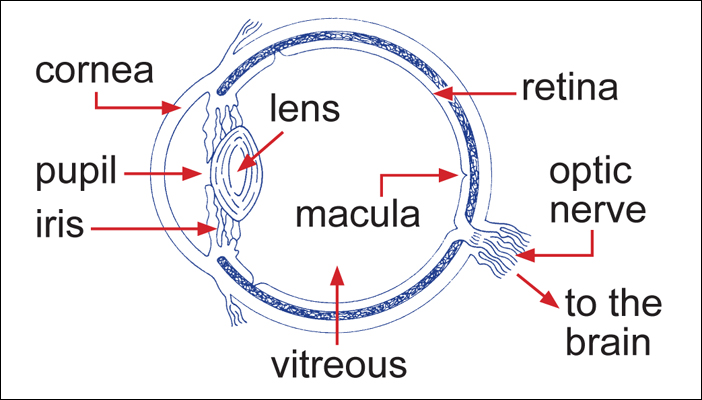
\includegraphics{figures/eye}
  \caption{A simple schematic diagram of the layout of the eye.}
  \label{fig:eye_simple}
\end{figure}

The cornea of the eye is a transparent layer around 0.6mm thick
which curves around the iris of the eye as well as its anterior
chamber.\cite{yaylali1997corneal,thoft1983x,patel1994refractive}
With a mean refractive index of around 1.4 (about the same as water),
the cornea allows plenty of light to pass through, but refracts as a
convergent lens due to its convex, shape. \Eref{eq:refractive} shows
Snell's Law of refraction for a light wave passing through two
different isotropic materials which have refractive indices $n_1$
and $n_2$, respectively.

\begin{figure}[htbp]
  \centering
    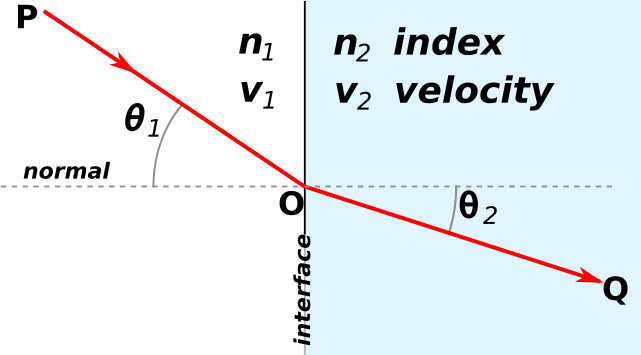
\includegraphics{figures/snells}
  \caption{Snell's law for diffraction at an interface where $n_1$ \textless $n_2$}
  \label{fig:snell}
\end{figure}

The angle $\theta_1$ is normal to the boundary between $n_1$ and $n_2$
and the angle $\theta_2$ is normal to the boundary between $n_2$ and $n_1$
as shown in \fref{fig:snell}

\begin{equation}
n_1\sin\theta_1=n_2\sin\theta_2
\label{eq:refractive}
\end{equation}

The radius of the human cornea tends to decrease with age and the cornea
itself, takes on a more spherical shape.\cite{guirao2000optical} Its
outermost surface is made of epithelial cells which are continuously lost
and replaced.\cite{jester1999cellular,hassell2010molecular} The reproduction
of cells is facilitated in part by tear ducts, which  serve to moisten the
eyes and remove harmful bacteria.\cite{holly1977tear}

There is a small circular opening in the iris, (the coloured section of
the eye) the pupil, has an aperture which dilates to allow an appropriate
amount of refracted light to pass through the lens. Light is refracted
once again through the lens converges towards a focal point on the back
of the eye. The lens makers expression in \eref{eq:lens_makers} is an
expression described by the diagram in \fref{fig:convergent_lens} which
shows light passing through a convex lens for calculating the focal point,
$f$ of distances $S_1$ and $S_2$ either side of a given convex lens.
\cite{greivenkamp2004field}

\begin{equation}
\frac{1}{S_1} + \frac{1}{S_2} = \frac{1}{f}
\label{eq:lens_makers}
\end{equation}

\begin{figure}[htbp]
  \centering
    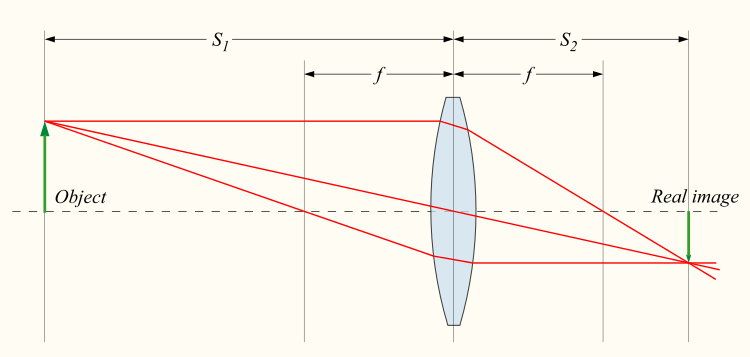
\includegraphics{figures/convergent_lens2}
  \caption{light passing through a convex lens for calculating the focal
  point, $f$ of distances $S_1$ and $S_2$ either side of a given convex lens.}
  \label{fig:convergent_lens}
\end{figure}

A ciliary body of tissue made up of fiber and muscle which accommodates the
lens and secretes a fluid, known as Aqueous Humour into a canal that flows
around the circumference of the eye called the Scleral Venous Sinus.
\cite{bill1970effects,dvorak1934schlemm}

When it becomes necessary to focus on objects at short distances, the
ciliary body muscles contract and suspensory ligaments attached to the
posterior chamber and the posterior lens to become taut, causing the
lens to become somewhat flatter, in response to applied contractile
forces. When objects are far away the light is more parallel to the lens'
principle axis, the muscles relax and suspensory ligaments attached to
the posterior chamber and the posterior lens so that it is no longer being
accommodated so it can take on a more rounded shape.

Photons of light are refracted out of the lens, before they pass through
a clear substance called the vitreous chamber and land onto the retina,
which is also transparent. A diagram indicating the optic axis and
visual axis is shown in \fref{fig:optic_axis}.

\begin{figure}[htbp]
  \centering
    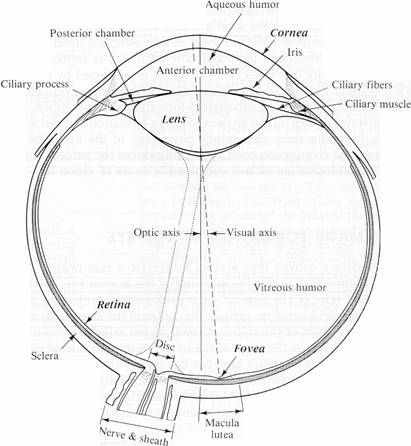
\includegraphics{figures/eye_diagram}
  \caption{A diagram of the eye showing of the visual
   and optic axis, the cornea, the retina and the fovea}
  \label{fig:optic_axis}
\end{figure} 

The retina is a membrane which covers the entire receptive field of
vision, it is part of the central nervous system.\cite{rogers1983neurite}
Just behind the retina are ganglion cells, biploar cells, cones and rods.
These are supported by pigment epithelium cells and the coroid, a vascular
bed of tissues which supply the retina with blood and removes toxins.
\cite{lutty1996localization} A schematic overview of the core retinal
constitution is given in \fref{fig:retina}

\begin{figure}[htbp]
  \centering
    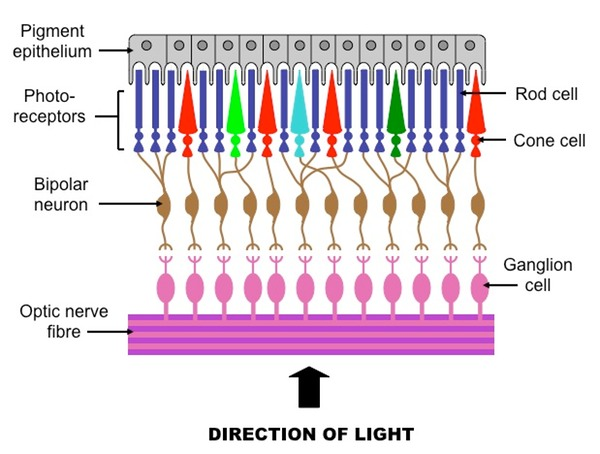
\includegraphics{figures/retina}
  \caption{A schematic diagram of the retina with the direction of light indicated
  as being from the bottom upwards direction.}
  \label{fig:retina}
\end{figure}

There are around 0.7 to 1.5 million ganglion cells in a normal human retina.
\cite{curcio1990topography}. Retinal ganglion cells are  they are part of
the system which passes electrical signals to the brain.
\cite{meyer1995characterization} Cones and rods are photoreceptors that ensure
that light is converted into electrical signals which are transmitted to the
brain from the optic nerve, via bunches of ganglion nerves.

Whilst cones are not particularly sensitive to light, they do aid to visual
acuity by granting us colour vision.\cite{bowmaker1980visual} Conversely, cones
which have a region of pigments around $1\mu{m}$, are particularly sensitive,
even to single the pressure exerted by single photons of light at a time,
so they tend to be located around the periphery of the receptive field of
the retina.\cite{liebman1964sensitive,baylor1979responses} 
Most of the retinal cones are located around a circular trough in the
receptive field, called the fovea centralis which is located at the center
of the macular.\cite{hendrickson1994primate} it is the most sensitive part
of the eye. The fovea has an apparent dip, because unlike the periphery,
there are neurons situated behind it, Neurons have axons that allow electrical
signals travel to the optic nerve so they can be interpreted by the brain but
as the fovea is a particularly sensitive aid to colour vision and acuity,
axons of neurons would get in the way if they were located directly behind it.

A healthy and normal eye will pick up red, green and blue so that the brain
can interpret the full spectrum of colours, including white. \fref{fig:wavelengths}
shows normalised absorbency against wavelength for red, green and blue cones
and rods (which cannot differentiate between colours), in an average, human eye.
The range of human visual spectrum of of light lies roughly between 390nm
and 700nm.\cite{starr2010biology}.

\begin{figure}[htbp]
  \centering
    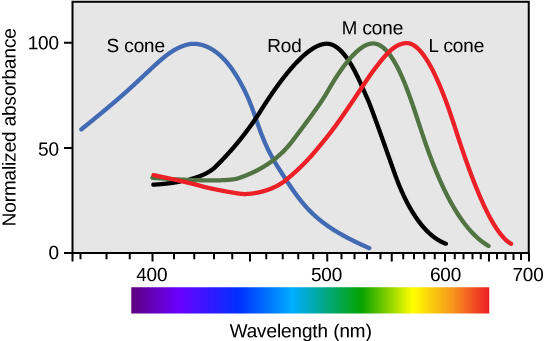
\includegraphics{wavelengths}
  \caption{Normalised absorbency vs. wavelength, for an average eye.}
  \label{fig:wavelengths}
\end{figure}

\section{Development, Dysfunction, Ageing and Disease}

During the early stages of development in babies, there is a steady
increase of a lubricating substance called glycosaminoglycan hexosamine,
in the cornea which reaches an increase plateau at around 2 years of age.
\cite{praus1975glycosaminoglycans}

Some men are born with limited functionality in cones which are
sensitive to particular frequencies of light.\cite{george1996clinical}
If all the eye cones are not working then this causes blindness
to occur but if only some types of cones have limited functionality
as photoreceptors this causes a less serious impairment, commonly
referred to as "colour blindness".

As people age, ciliary muscles weaken and this impairs the ciliary
muscles' ability to accommodate the lens and the result of this is
difficulty focusing on objects which are close by.
\cite{fisher1985ciliary}

Age related Macular degeneration of pigment cells and decreases in
Equatorial rods and ganglion cell rates are common problems affecting
central vision.\cite{gao1992aging} Macular degeneration in particular,
accounts for 95\% of blind and partial sightedness registrations in the
UK and particularly affects women.\cite{o1998age,klein2005complement}
There are two main forms of macular degeneration, non-exudative (dry)
and exudative (wet). The phenotypes in on-exudative macular degeneration
are atrophic and neovascular respectively.\cite{kuno2011dry} In
non-exudative macular degeneration, deposits build up behind the retina
resulting in its progressive thinning or scarring, with respect to time.
Exudative macular degeneration is caused by leaking of blood vessels
which causes swelling.

Preliminary studies indicate that the thickness of the coroid decreases
with age and although little is understood about how this may affect
central vision in macular degeneration, some studies have found
coroid thickness to be a predictor for open angle glaucoma which
is yet another leading cause of blindness.
\cite{margolis2009pilot,gordon2002ocular}

Glaucoma is caused by various malfunctions of aqueous humour drainage
which can lead to excessive interocular pressure bringing about damage
to the optic nerve and other vital members of the optical system.
\cite{distelhorst2003open} Open angle glaucoma happens gradually,
affecting the peripheral vision at first and progresses on to impair
central vision over time. For early diagnosis of open angle glaucoma
the relationship between interocular pressure and visual field decay
is examined by specialists to determine whether any abnormalities are
apparent so that it may be treated before permanent field damage occurs.
\cite{goldmann1972open}

Retinopathy is another common disease but one which can affect people of
all ages, by attacking the retina, A common indicator of non-proliferative
retinopathy is macular edema, symptomatic blurred vision arising from
abnormal fluid leakage and swelling in the macular from the retina's
blood vessels causing the the retina to thicken.\cite{hee1995quantitative}
Macular edema is the common cause of visual degeneration in people with
diabetes which can significantly increases a person's chance of developing
retinopathy as the diabetes progresses.\cite{klein1984wisconsin} Proliferative
diabetic retinopathy is caused by blockages in blood vessels which can can
starve the retina of oxygen. The retina responds to this by attempting to
grow blood vessels of its own, however they tend to be abnormal and hinder
fluid secretion and leak blood into the vitreous humour. Symptoms of
prolific retinopathy do not usually occur until damage has already been
done and in that case a sufferer would experience seeing "floaters",
"shadows" and loss of vision.
